\documentclass[aspectratio=169,11pt]{beamer}
\usepackage[T1]{fontenc}
\usepackage{lmodern}
\usepackage{amsmath,amssymb,booktabs,array}
\usepackage{graphicx}
\usepackage{appendixnumberbeamer}
\definecolor{ink}{HTML}{153349}
\definecolor{teal}{HTML}{087F8C}
\definecolor{muted}{HTML}{566675}
\definecolor{pale}{HTML}{EDF5F6}
\setbeamercolor{normal text}{fg=ink,bg=white}
\setbeamercolor{structure}{fg=teal}
\setbeamercolor{frametitle}{fg=ink}
\setbeamercolor{block title}{fg=teal,bg=white}
\setbeamercolor{block body}{fg=ink,bg=white}
\setbeamerfont{frametitle}{size=\large,series=\bfseries}
\setbeamerfont{block title}{size=\normalsize,series=\bfseries}
\setbeamertemplate{navigation symbols}{}
\setbeamersize{text margin left=8mm,text margin right=8mm}
\setbeamertemplate{frametitle}[default][left]
\addtobeamertemplate{frametitle}{\vspace{2mm}}{}
\pdfstringdefDisableCommands{\def\translate#1{#1}}
\setbeamertemplate{footline}{%
  \hspace{8mm}\color{muted}\fontsize{6.5}{8}\selectfont
  TI tuned receiver\hfill Internal working presentation · 7 November 2026
  \hspace{5mm}\insertframenumber\hspace{8mm}\vspace{3mm}}
\setlength{\parskip}{5pt}
\setlength{\abovedisplayskip}{6pt}
\setlength{\belowdisplayskip}{6pt}
\newcommand{\source}[1]{\vfill{\color{muted}\fontsize{6.5}{8}\selectfont #1\par}}
\newcommand{\smalltext}{\fontsize{9}{11}\selectfont}
\newcommand{\eps}{\varepsilon}
\newcommand{\gain}{G}
\title{The cortical column as a tuned receiver}
\subtitle{A network mechanism for temporal-interference stimulation}
\author{G. Ruffini and colleagues}
\date{7 November 2026}
\hypersetup{pdftitle={TI: the cortical column as a tuned receiver},
pdfauthor={Giulio Ruffini and colleagues},pdfsubject={Main results of TN0484, draft28, with verified November 6 FEM additions}}

\begin{document}

\begin{frame}[t]
{The cortical column as a tuned receiver}
\vspace{0mm}
{\color{teal}\large A network mechanism for temporal-interference stimulation}

\vspace{2mm}
{\smalltext G. Ruffini, R. Salvador, B. Mercadal, R. de Palma Aristides,\\
F. Castaldo, N. Grossman, S. Canals, C. Mirasso}

\vspace{1mm}
Two carriers at angular frequencies $\omega_1$ and $\omega_2$ can generate a
neural response at their difference $\Omega=|\omega_2-\omega_1|$, absent from the applied spectrum.

\begin{columns}[T,onlytextwidth]
\column{.31\textwidth}
\begin{block}{Access}
The field produces local membrane polarization.
\end{block}
\column{.31\textwidth}
\begin{block}{Detection}
Nonlinearity generates beat and steady sources.
\end{block}
\column{.31\textwidth}
\begin{block}{Amplification}
The circuit selects and amplifies its received input.
\end{block}
\end{columns}

\vspace{2mm}
These stages act in series. A large circuit response can coexist with a small local source.
\source{TN0484 / WP0185, draft28. The physiological transfer from a kHz field to the detector remains uncalibrated.}
\end{frame}

\begin{frame}[t]{The weak beat follows the carrier product}
Let $s(t)=\eps_1\cos\omega_1t+\eps_2\cos\omega_2t$ be the polarization entering
a static rate curve $\sigma$ at operating voltage $v^*$.
\[
\sigma(v^*+s)\simeq\sigma(v^*)+\sigma'(v^*)s+\tfrac12\sigma''(v^*)s^2.
\]
The signed coefficient of $\cos\Omega t$ is
\[
\color{teal}Y_\Omega=\tfrac12\sigma''(v^*)\eps_1\eps_2.
\]
Envelope-based targeting uses $2\min(|\eps_1|,|\eps_2|)$, with a different amplitude dependence.

\vspace{2mm}
For fixed polarization profiles $P_j(\mathbf r)$, let
$\eps_j=I_jP_j(\mathbf r)$, where $I_j$ is applied current. At fixed neural state,
\[
Y_\Omega(\mathbf r)\propto I_1I_2\,P_1(\mathbf r)P_2(\mathbf r).
\]
Changing the current ratio rescales the quadratic beat map; it cannot move its normalized pattern.
\source{Weak-field expansion; fixed coupling and operating state. The common current-product factor also survives bilinear multicompartment detection.}
\end{frame}

\begin{frame}[t]{The same detector generates a signed steady source}
\[
\color{teal}Y_{\rm DC}=\frac{\sigma''(v^*)}{4}
\left(\eps_1^2+\eps_2^2\right).
\]
This is a DC-like detector output even though the applied field has no direct-current component.
For a static detector its sign follows curvature; reversing either carrier leaves it unchanged.

\vspace{1mm}
Define the mean-square polarization $\mathcal I=(\eps_1^2+\eps_2^2)/2$.
If each $\eps_j$ is harmonic,
\[
\nabla^2\mathcal I=|\nabla\eps_1|^2+|\nabla\eps_2|^2\geq0.
\]
Therefore $\mathcal I$ has no strict interior maximum. The same holds for
$|Y_{\rm DC}|$ when the detector coefficient is spatially constant.

\vspace{2mm}
Spatial variation in detector state can still select where the steady response is largest.
\source{Maximum restriction: homogeneous, isotropic, source-free tissue with spatially fixed coupling. The circuit's mean-rate response is distinct from this source.}
\end{frame}

\begin{frame}[t]{Current ratio separates the spatial predictions}
\begin{columns}[T,onlytextwidth]
\column{.32\textwidth}
At fixed total current, changing $2+2$ to $1+3$ mA gives different outcomes.

The quadratic beat falls by 25\% with its normalized pattern unchanged.

The envelope centroid moves 2.5 mm anteriorly; the mean-square centroid moves 4.5 mm posteriorly.

{\smalltext Centroids use the highest 10\% of nodes within the hippocampal region of interest (ROI).}
\column{.66\textwidth}
\centering
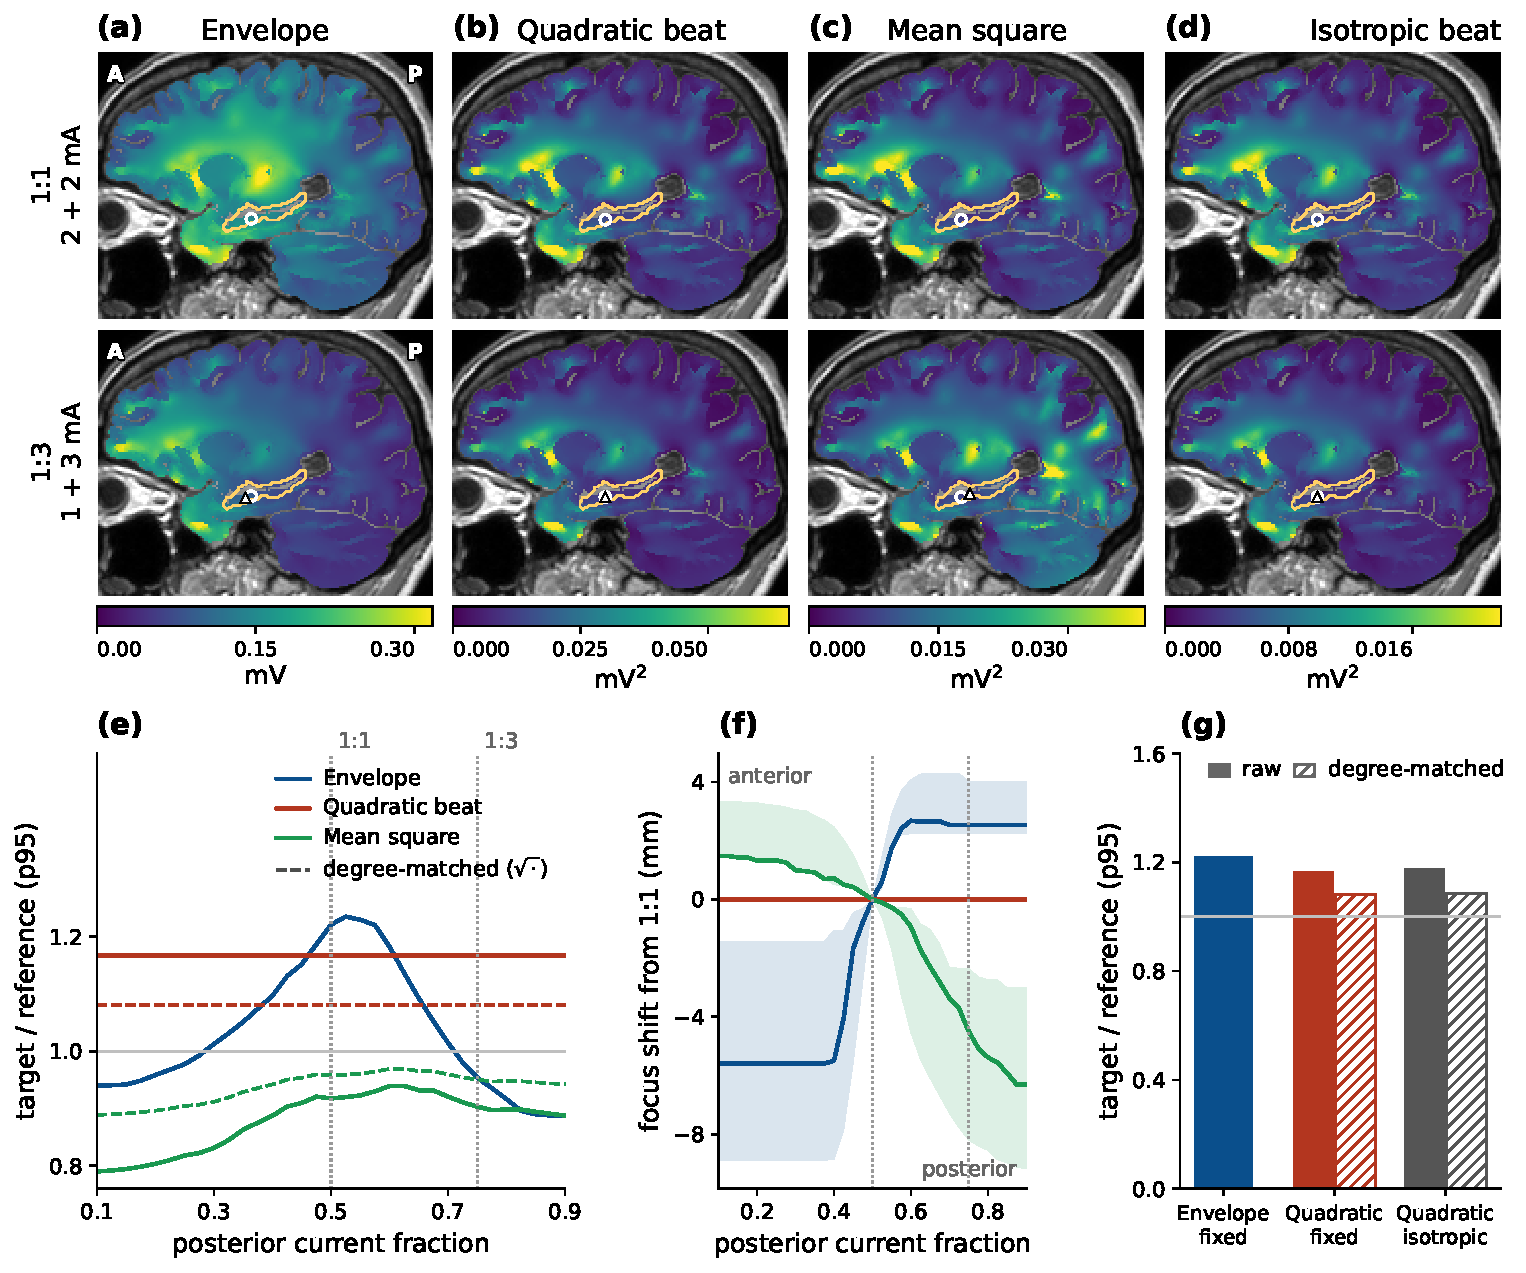
\includegraphics[width=\linewidth,trim=0bp 277bp 181bp 0bp,clip]{figures/fig_fem.pdf}
\end{columns}
\source{One IXI002 head, Violante montage. Orientation maximizes the balanced envelope and is then held fixed. Opposite centroid motion is geometry-dependent; these are not global exposure maxima. MRI: IXI dataset, CC BY-SA 3.0.}
\end{frame}

\begin{frame}[t]{GM-only contrasts limit hippocampal beat selectivity}
\begin{columns}[T,onlytextwidth]
\column{.55\textwidth}
\small
\renewcommand{\arraystretch}{1.3}
\begin{tabular}{@{}lrr@{}}
\toprule
ROI p95 / reference p95 & 1:1 & 1:3\\
\midrule
Envelope & 1.09 & 0.84\\
Quadratic beat & 0.94 & 0.94\\
\quad degree-matched & 0.97 & 0.97\\
Mean square & 0.71 & 0.76\\
\quad degree-matched & 0.85 & 0.87\\
\bottomrule
\end{tabular}

\vspace{3mm}
{\smalltext Gray-matter-only hippocampal ROI: 1,174 nodes. Reference: all gray matter outside the ROI. Degree matching takes the square root of each map before computing contrasts.}
\column{.41\textwidth}
At 1:1, only the envelope exceeds one; at 1:3, none does.

Mean square rises 17.2--29.7\% across eight montage, label, and tissue variants; the envelope falls 43.9--46.2\%.

{\smalltext In the baseline GM+WM ROI, mean square rises at 86.3\% of nodes and the envelope at 0.13\%.}
\end{columns}
\source{Ricardo's November 6 outputs, PR \#2 at 6ade413; checked against the JSON. Included in draft28. One head; geometric maps precede detector and circuit weighting.}
\end{frame}

\begin{frame}[t]{Recurrence changes gain while detection stays fixed}
\begin{columns}[T,onlytextwidth]
\column{.48\textwidth}
The Jansen--Rit (JR) sweep pins the operating voltage at $v^*=8.30$ mV, keeping detection fixed.

Near a Hopf bifurcation,
\[
|\gain(\Omega)|\propto\frac1\gamma,
\]
where $\gamma>0$ is modal damping. Finite forcing eventually saturates the response.

Direct transcranial alternating-current stimulation (tACS) shares this amplifier at the same state and readout.
\column{.49\textwidth}
\centering
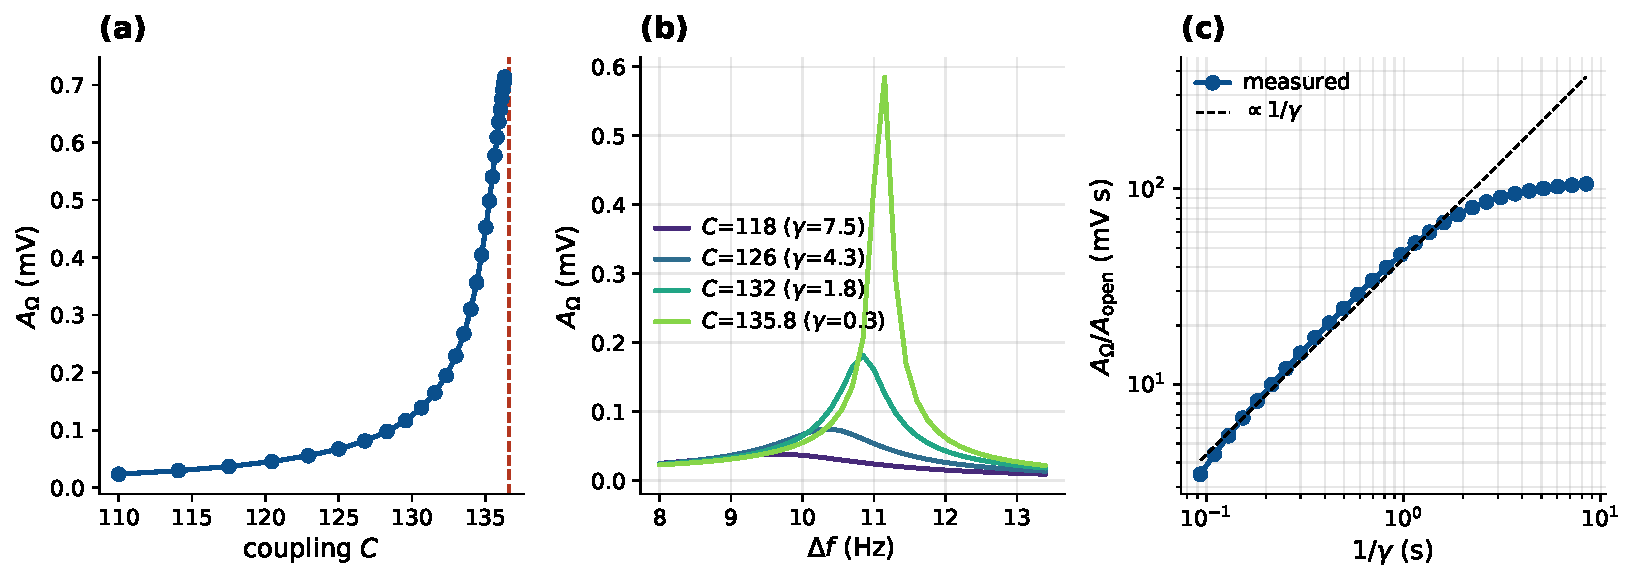
\includegraphics[height=48mm,trim=523bp 0bp 0bp 0bp,clip]{figures/fig_jcurve.pdf}\par
{\fontsize{8}{10}\selectfont $A_\Omega$: beat-frequency voltage amplitude.\\
$A_{\rm open}$: open-loop rate-source amplitude.}
\end{columns}
\source{JR amplitude-modulated surrogate, pinned-state experiment. In the weakly driven regime, the response is mainly beat-locked population-rate modulation, with little mean-rate change.}
\end{frame}

\begin{frame}[t]{Dynamic detection can reverse the static sign prediction}
\begin{columns}[T,onlytextwidth]
\column{.58\textwidth}
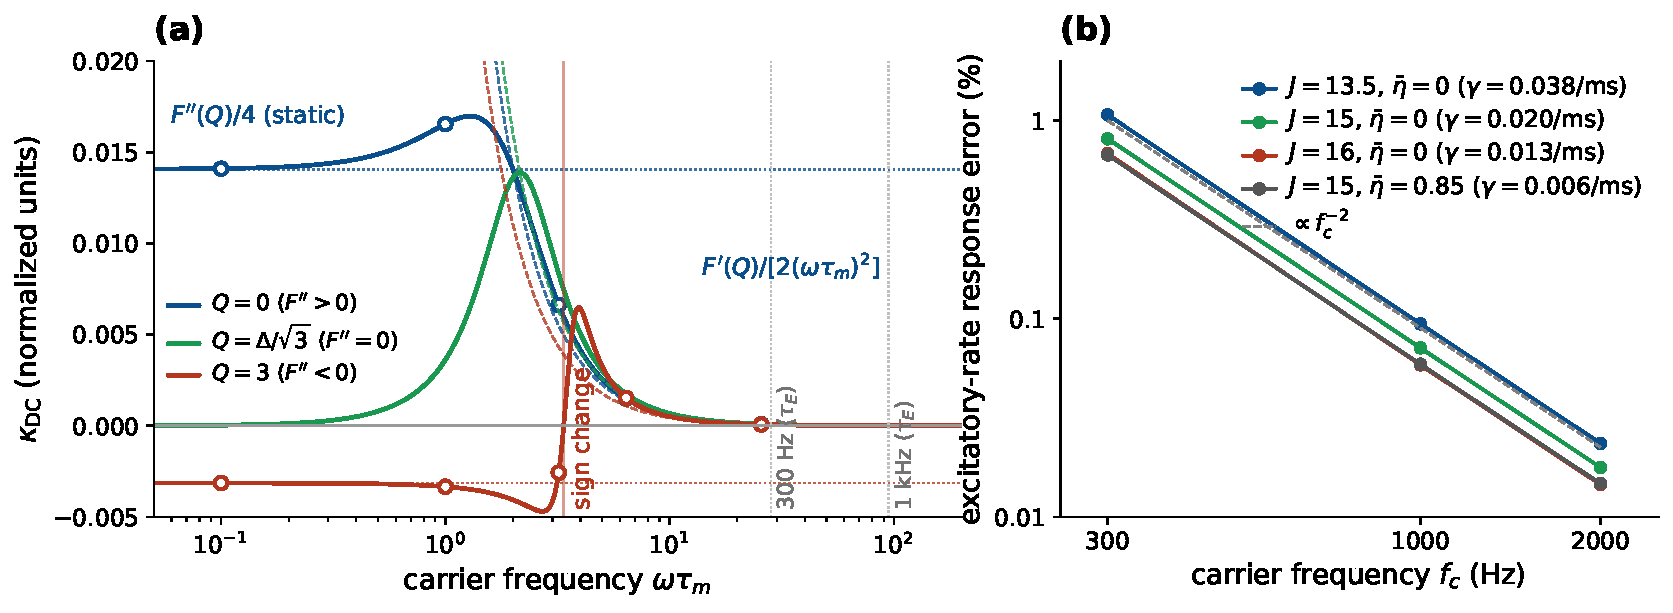
\includegraphics[width=\linewidth,trim=0bp 0bp 354bp 0bp,clip]{figures/fig_mpr_crossover.pdf}
\column{.39\textwidth}
\small
For input $I_{\rm ac}\cos\omega t$, define the steady rate shift by
\[
\delta\bar r=I_{\rm ac}^2\kappa_{\rm DC}/\tau_m.
\]
Its slow- and fast-carrier limits are
\[
\kappa_{\rm DC}\longrightarrow\frac{F''(Q)}4,
\qquad\omega\tau_m\ll1,
\]
\[
\kappa_{\rm DC}\sim\frac{F'(Q)}{2(\omega\tau_m)^2},
\quad\omega\tau_m\gg1.
\]
\end{columns}
The fast-carrier contribution is positive even where static curvature is negative.
\source{Quadratic integrate-and-fire (QIF) mean field. $F(Q)$: dimensionless steady rate at drive $Q$; $\tau_m$: membrane time; $\omega$: carrier angular frequency. Weak local rectification at fixed synaptic input. $\Delta$ in the plot is the drive-distribution half-width.}
\end{frame}

\begin{frame}[t]{TI sources are quadratic; direct sources are linear}
For weak balanced TI, each carrier has polarization amplitude $\eps$.
A direct input of the same amplitude at the same detector entry gives:
\[
|Y_{\rm TI}|=\tfrac12|\sigma''|\eps^2,
\qquad |Y_{\rm direct}|=\sigma'\eps.
\]
Compare the steady source with transcranial direct-current stimulation (tDCS),
and the beat source with tACS.

\vspace{2mm}
\begin{columns}[c,onlytextwidth]
\column{.48\textwidth}
\[
\frac{|Y_{\rm TI}|}{|Y_{\rm direct}|}
=\frac{|\sigma''|}{2\sigma'}\eps.
\]
\column{.48\textwidth}
\centering
\renewcommand{\arraystretch}{1.25}
\begin{tabular}{@{}rr@{}}
\toprule
Polarization per input & Source ratio\\
\midrule
0.1 mV & 1.6\%\\
0.3 mV & 4.8\%\\
\bottomrule
\end{tabular}
\end{columns}

\vspace{0mm}
At the JR state studied, TI sources are approximately 2--5\% of the corresponding direct sources.
\source{$\sigma'=0.4745$ s$^{-1}$mV$^{-1}$; $\sigma''=-0.1508$ s$^{-1}$mV$^{-2}$. Local source comparison before feedback, not a clinical-effect ratio. Matching total peak polarization instead halves the ratio.}
\end{frame}

\begin{frame}[t]{Carrier access sets a conditional kHz input budget}
\begin{columns}[T,onlytextwidth]
\column{.55\textwidth}
For carrier frequency $f$ and per-tone field $E$, a first-order access filter gives
\[
\eps=\frac{\lambda_0 E}{\sqrt{1+(2\pi f\tau)^2}}.
\]
Assume access time $\tau=0.2$ ms and low-frequency coupling $\lambda_0=0.5$ mV/(V/m).

At 2 kHz and $E=0.5$ V/m, the beat source matches a direct input of magnitude \textbf{\mbox{1.36\,$\mu$V}}.
\column{.42\textwidth}
\centering
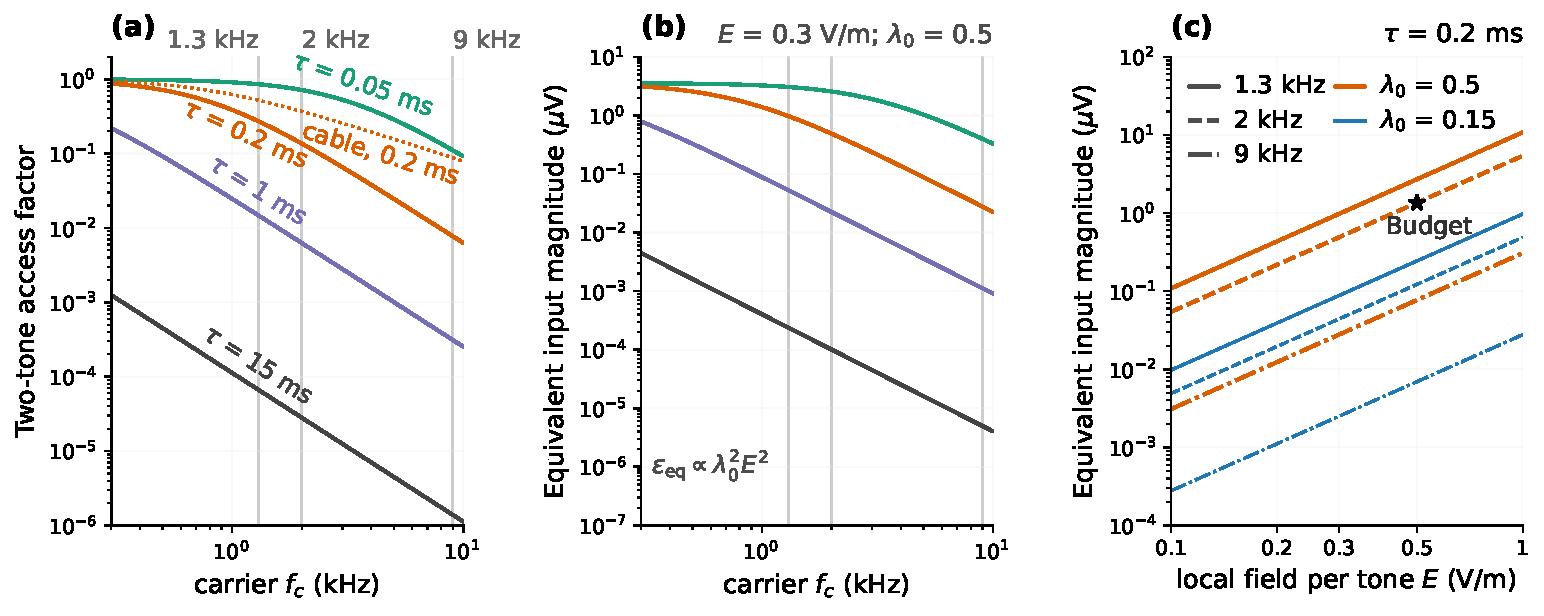
\includegraphics[height=51mm,trim=495bp 0bp 0bp 0bp,clip]{figures/fig_feasibility_khz.pdf}
\end{columns}
\source{Static JR chain; equivalent input $\eps_{\rm eq}=Y_\Omega/\sigma'$. These access and coupling values are assumptions, not tissue calibration. Reducing $\lambda_0$ to 0.15 multiplies the source by 0.09.}
\end{frame}

\begin{frame}[t]{A steady shift can induce gamma without a beat}
The excitatory--inhibitory QIF mean field compares TI with an unmodulated carrier at equal root-mean-square (RMS) input current.
\begin{columns}[T,onlytextwidth]
\column{.49\textwidth}\centering\small\color{teal}TI per-tone input amplitude 10
\column{.49\textwidth}\centering\small\color{teal}TI per-tone input amplitude 35
\end{columns}
\vspace{1mm}
\centering
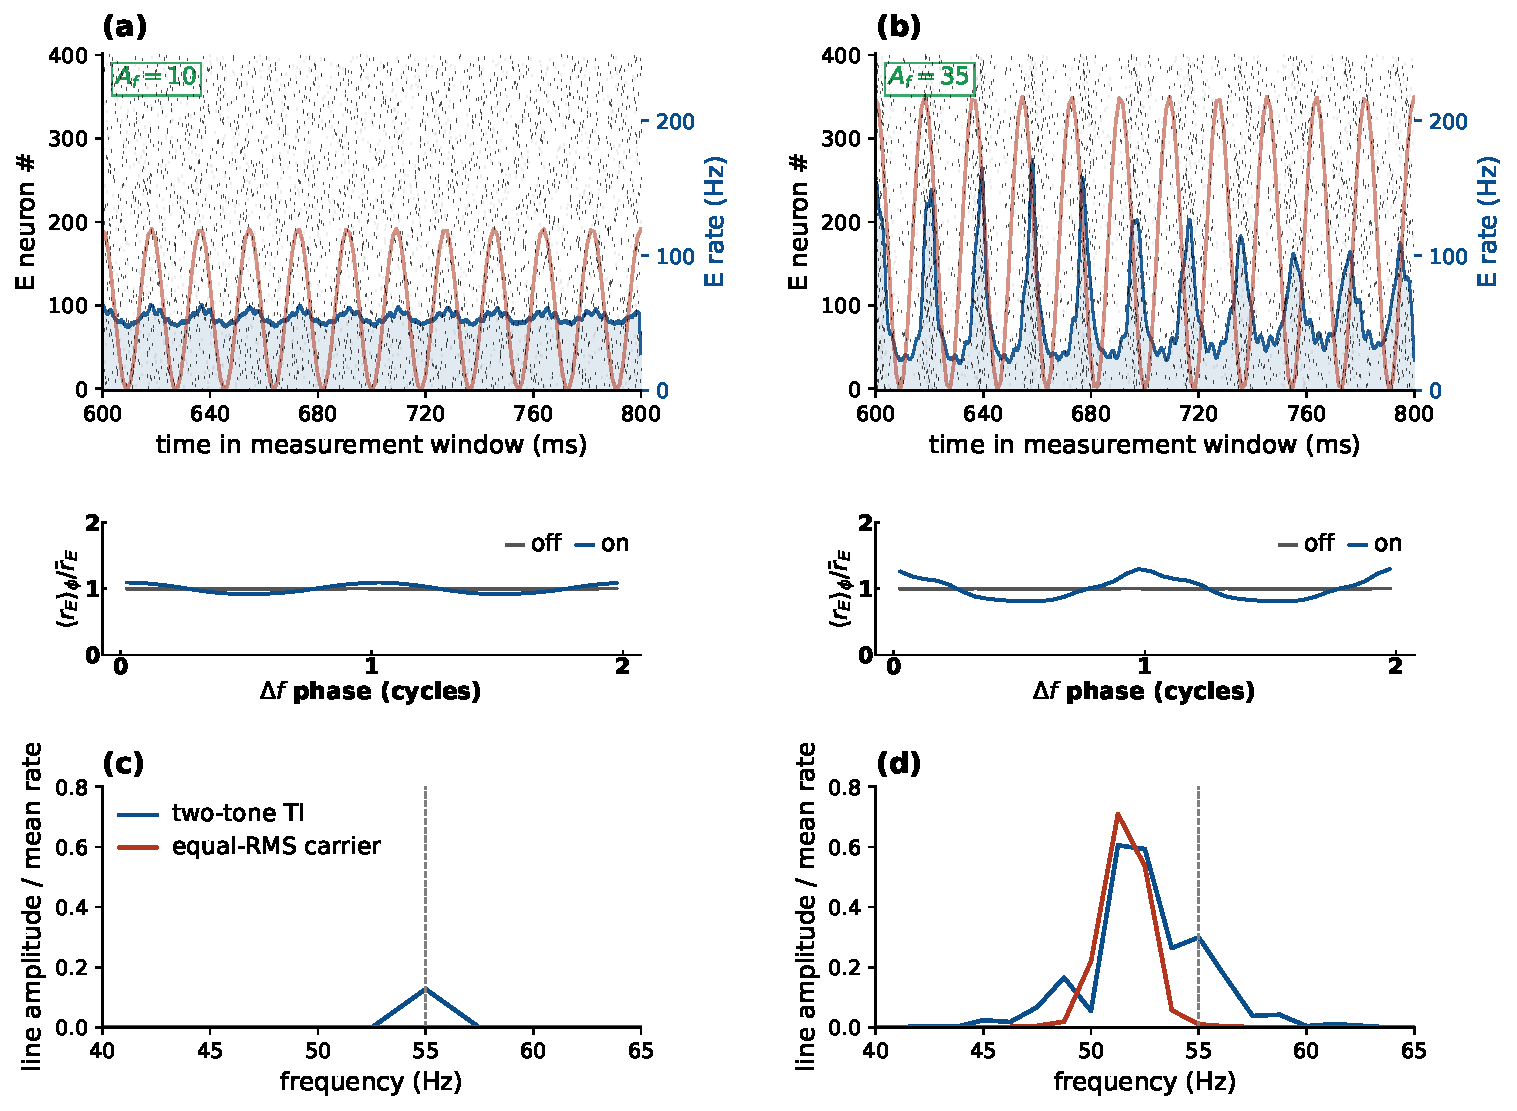
\includegraphics[width=.90\linewidth,trim=0bp 0bp 0bp 354bp,clip]{figures/fig_qif_regimes.pdf}
\par\raggedright
Both stimuli induce gamma near 51 Hz at larger input; TI also has a 55 Hz beat.
The unmodulated carrier separates steady-shift responses from beat-dependent ones.
\source{300 Hz carrier; input current in model units. Mean-field controls only. Finite-network modulation depth remains unconverged (backup B1). Gamma induction is not evidence of entrainment.}
\end{frame}

\begin{frame}[t]{TI combines local mixing with a state-dependent amplifier}
Weak nonlinear detection produces a beat and a steady source together.
At fixed geometry and neural state, the carrier product sets the beat map;
changing the current ratio rescales that map without moving it.

\medskip
The receiving circuit sets the gain, which TI shares with direct tACS.
A sufficiently large steady shift can itself induce oscillations, while dynamic
detection can reverse the sign predicted by a static rate curve.

\medskip
Physiological source strength remains unresolved at kHz frequencies.
Measure local carrier polarization, vary the two amplitudes independently,
and compare beat and steady responses with an equal-RMS carrier across circuit states.
\source{The models establish these mechanisms and their conditions. The head-model results illustrate geometry in one subject; they do not establish physiological deep selectivity.}
\end{frame}

\appendix
\begin{frame}[t]{B1. Finite-network convergence remains incomplete}
\begin{columns}[T,onlytextwidth]
\column{.38\textwidth}
The theta formulation removes the finite spike-reset lag. Population-size sensitivity remains.

Doubling the population changes modulation depth by $-11.9\%$, beyond the prespecified 5\% tolerance.

Time-step and window checks pass. The joint population/time-step limit remains untested.
\column{.59\textwidth}
\small
\renewcommand{\arraystretch}{1.35}
\begin{tabular}{@{}lr@{}}
\toprule
Weak-input condition & Depth\\
\midrule
QIF cutoff $V_{\rm peak}=100$ & 0.093\\
QIF cutoff $V_{\rm peak}=200$ & 0.127\\
QIF cutoff $V_{\rm peak}=400$ & 0.139\\
Cutoff-free, $N=8{,}000$ & 0.156\\
Cutoff-free, $N=16{,}000$ & 0.137\\
Exact mean field & 0.128\\
\bottomrule
\end{tabular}
\end{columns}
\source{Depth: rate lock-in amplitude divided by mean rate. $V_{\rm peak}$: numerical spike cutoff in model voltage units; $N$: neurons per population. No equal-RMS finite-network control was run.}
\end{frame}

\begin{frame}[t]{B2. The spatial checks compare distinct quantities}
\small
\renewcommand{\arraystretch}{1.2}
\begin{tabular}{@{}lccc@{}}
\toprule
GM-only ROI & Raw p95 contrast & Degree-matched p95 & Mean / reference p95\\
& 1:1 / 1:3 & 1:1 / 1:3 & 1:1 / 1:3\\
\midrule
Envelope & 1.086 / 0.839 & same & 0.757 / 0.547\\
Quadratic beat & 0.935 / 0.935 & 0.967 / 0.967 & 0.508 / 0.508\\
Isotropic beat & 0.943 / 0.943 & 0.971 / 0.971 & 0.512 / 0.512\\
Mean square & 0.715 / 0.765 & 0.845 / 0.874 & 0.396 / 0.462\\
\bottomrule
\end{tabular}

\vspace{3mm}
The eight mean-change variants combine two montages, two ROI labels, and two tissue selections.
They are all computed in one head. The focus-fraction choice changes centroids, not ROI means.

Across variants, mean square rises at 80.8--90.9\% of nodes; the envelope rises at 0--0.2\%.
These counts use equal node weights and each node's fixed balanced-envelope-maximizing orientation.

\source{Verified November 6 JSON outputs at 6ade413. The reported NPZ has not yet been received or independently validated. Reference: all gray matter outside the selected ROI.}
\end{frame}

\end{document}
